\section{事例筛选}\label{sec:evtsel}

%\section{粒子鉴别及筛选}

\subsection{粒子定义与重叠移除}\label{subsec:4w_obj_def}
%物理分析首先要明确事例内的各种粒子的定义(鉴别及筛选条件),而后才能进行事例级别的选择。
%粒子重建及鉴别遵循ATLAS一般流程,如章节\ref{sec:evt_reco}所述。
与前文\ref{sec:obj_tth}类似,首先须进行粒子定义和重叠移除。4W分析的粒子定义总结在表\ref{tab:4w_obj_def}。通过Baseline筛选的粒子会用于控制区域或者本底估计的研究,而通过Tight筛选的粒子才会作为信号区的输入。随后的重叠移除总结在表\ref{tab:4w_olr}。
\begin{table}[h]
\centering
\scalebox{0.9}{
\begin{tabular}{c|c| c c r r}
\hline
\hline
粒子     &\multicolumn{2}{c}{选择条件}    \\
\hline
         &Baseline     &Tight     \\
\cline{2-3}
\multirow{4}{*}{电子}  &\ET$>$ 10 GeV         &\texttt{TightLH} ID      \\
        &\abseta $<$ 2.47,排除1.37$<$\abseta$<$1.52 区间    &\texttt{FixedCutTight} \\
        &\texttt{LooseLH} ID, \texttt{Loose} isolation   &($\et^{\text{cone}20}/\pt<$0.06, $\pt^{\text{varcone}20}/\pt<$0.06)          \\
        &$|z_{0}\sin\theta| <$ 0.5~mm,$d_{0}/\sigma(d_{0}) <$ 5  &   \\
\hline
\multirow{4}{*}{$\mu$}  &\pt > 10 GeV         &\texttt{Tight} ID      \\
        &\abseta $<$ 2.5                      &\texttt{FixedCutTightTrackOnly} \\
        &\texttt{Loose} ID, \texttt{Loose} isolation   &($\pt^{\text{varcone}20}/\pt<$0.06)\\
        &$|z_{0}\sin\theta| <$ 0.5~mm,$d_{0}/\sigma(d_{0}) <$ 3  &   \\
\hline
\multirow{2}{*}{Jet}    &\multicolumn{2}{c}{\pt > 25 GeV, \abseta $<$ 2.5} \\
                        &\multicolumn{2}{c}{ |JVT|<0.59 if \pt < 60 GeV and \abseta $<$ 2.4}  \\
\hline
\met    &\multicolumn{2}{c}{$E_{\text{T}}^{\text{miss,TRK}}$}     \\
\hline
\hline
\end{tabular}}
\caption{4W物理分析粒子筛选条件总结}
\label{tab:4w_obj_def}
\end{table}


%\subsection{重叠移除}
%经过粒子基准(baseline)筛选之后,两个粒子之间的空间距离也许很小,这种情况有可能是因为同一个粒子信息被重建成两个(不同)粒子,
%为了消除这种重叠,专门的重叠移除(overlap removal)需要完成\cite{Adams:1743654}。
%该分析中的重叠移除总结如表\ref{tab:4w_olr}所示。
  \begin{table}
  \centering
  \small
  \begin{tabular}{|c|c|c|}
  \hline
               Keep        &Remove            &Cone size ($\Delta R$) \\
  %\hline
  %             electron    &tau               &0.2  \\
  %\hline
  %             muon        &tau               &0.2  \\
  \hline
               muon    &electron   &0.1 \\
  \hline
               electron     &electron(lower $p_T$)          &0.1 \\
  \hline
               electron    &jet               &0.3      \\
  \hline
               jet        &muon               &min(0.4, 0.04+10[GeV]/$p_T(\mu)$) \\
  \hline
  \end{tabular}
  \caption{Overlap removal in 4W analysis.}
  \label{tab:4w_olr}
  \end{table}

\clearpage
%\section{事例筛选}
\subsection{初步筛选}
完成粒子筛选和重叠移除之后,所选事例应当通过如下初步筛选条件:
\begin{itemize}
  \item \textbf{GRL (Good Run List)},ATLAS定义的物理分析可以使用的数据:\\
	\begin{tabular}{ll}
    2015年数据: & {\tt data15\_13TeV.periodAllYear\_DetStatus-v79-repro20-02} \\
                      & {\tt \_DQDefects-00-02-02\_PHYS\_StandardGRL\_All\_Good\_25ns.xml} \\
    %2016 data: & {\tt data16\_13TeV.periodAllYear\_DetStatus-v83-pro20-15} \\
    %                  & {\tt \_DQDefects-00-02-04\_PHYS\_StandardGRL\_All\_Good\_25ns.xml}
   2016年数据: & {\tt data16\_13TeV.periodAllYear\_DetStatus-v88-pro20-21} \\
                    & {\tt \_DQDefects-00-02-04\_PHYS\_StandardGRL\_All\_Good\_25ns.xml} \\
  \end{tabular}
  \item \textbf{事例清洁(Event cleaning criteria)}: 去除量能器信息不全的事例。%cleaning for Tile corrupted events, LAr noise bursts and corrupted data
  \item \textbf{初始顶点}: 事例至少有一个包含两条径迹的初始顶点。%详细可见\cite{vertex_ref}。%events are required to contain at least one primary vertex with $\ge2$ associated tracks. The detailed selection on the vertex can be found in~\cite{vertex_ref}
  \item \textbf{触发判选} \\
   2015年数据:
    \begin{itemize}
     \item 单轻子触发: HLT\_mu20\_iloose\_L1MU15 || HLT\_mu50 || HLT\_e24\_lhmedium\_L1EM20VH ||
     HLT\_e60\_lhmedium || HLT\_e120\_lhloose 
     \item 双轻子触发: HLT\_2e12\_lhloose\_L12EM10VH || HLT\_e17\_lhloose\_mu14 || HLT\_mu18\_mu8noL1
    \end{itemize}
  2016年数据:
  \begin{itemize}
    \item 单轻子触发: HLT\_mu24\_ivarmedium || HLT\_mu50 || HLT\_e24\_lhtight\_nod0\_ivarloose ||
      HLT\_e60\_lhmedium\_nod0 || HLT\_e140\_lhloose\_nod0  
    \item 双轻子触发: HLT\_2e17\_lhvloose\_nod0 || HLT\_e17\_lhloose\_nod0\_mu14 ||\\
     HLT\_mu22\_mu8noL1 
  \end{itemize}
 需要指出的是,与数据一样,MC样本也应当满足以上触发条件,其相应的触发效率修正已添加到每个样本事例中。
  \item 选择通过章节~\ref{subsec:4w_obj_def}所述的粒子。
  \item \textbf{轻子数}
	\begin{itemize}
	      \item 两个相同电荷的轻子,可有效压低$Z/\gamma^*$和QCD本底。
	      \item 每个\texttt{tight}电子应当满足\texttt{ChargeIDBDTTight}> 0.067,此变量用于压低电荷误判电子。
	      \item 至少有一个轻子应当能匹配以上任一或多个trigger,除此之外,领头轻子\pt 应大于30 GeV,次领头轻子大于20 GeV。
	\end{itemize}
  \item 排除掉任何含有\bjet 的事例。
  \item $E_{\text{T}}^{\text{miss,TRK}}$> 10 GeV。
  \item 因为Drell-Yan过程目前并不能被MC很好模拟,所以为了避免此问题,双轻子不变质量应大于15 GeV。
  \item 为了压低来自于$Z$+jets过程的本底(电荷误判),须满足$|M(\ell\ell)-M(Z)|>$10~GeV条件。
  \item 喷注数的要求依赖于质量点的选择,低(高)质量点要求至少2 (3)个喷注。此项会在~\ref{subsubsec:hh_optimization}深入讨论。
\end{itemize}

以上的事例筛选过程总结在表~\ref{tab:4w_evt_presel}。最后,通过以上筛选条件的事例根据轻子味道分为三个分析道,为$ee$,
$\mu\mu$和$e\mu$。表~\ref{tab:presel_cutflow_smhh}展示了标准模型希格斯粒子对信号经过以上一系列条件时的事例数和效率变化,
此处对应亮度为36.1 fb$^{-1}$,截面($gg\rightarrow hh$)为33.4 fb。图~\ref{fig:eff_pre_sel_hh}(图~\ref{fig:eff_pre_sel_SS})展示所有$hh$ ($SS$)信号样本经过初步筛选之后的效率,随着$m_X$或者$m_S$的增加,效率相应增加(对于$SS$,在$m_X=340~\text{GeV}, m_S=135~\text{GeV}$质量点的效率下降是因为从此点开始要求至少三个喷注);$e\mu$道具有最大的效率值,$\mu\mu$次之,$ee$最低,这是因为理论上$e\mu$的分支比是其他两个道的两倍,以及$\mu$比$e$具有更好的鉴别效率。
\begin{table}
\centering
\small
\begin{tabular}{c|ccccccccccc}
\hline
\hline
\multirow{12}{2cm}{Pre-selections} &GRL \\
                                  &Event clean criteria\\
                                  &Pass any trigger applied \\
                                  &Select objects following object definitions\\
                                  &Overlap removal \\
                                  &Two tight same-signed leptons, with at least one trigger matched \\
                                  &$p_T(\ell_1) >30$~GeV, $p_T(\ell_2)>20$~GeV \\
                                  &$b$ veto \\
                                  &$E_T^{miss}>$10~GeV \\
                                  &$M(\ell\ell)>$15~GeV \\
                                  &$|M(\ell\ell)-M(Z)|>$10~GeV in $ee$ channel\\
                                  &$N_\text{jet}\geq$2(3) \\
\hline
\hline
\end{tabular}
\caption{4W事例初步筛选条件。}
\label{tab:4w_evt_presel}
\end{table}

\begin{table}
\centering\small
\scalebox{0.9}{
\begin{tabular}{c|ccc|ccc}
\hline
\hline
Cut flow &\multicolumn{3}{c|}{Event yield}&\multicolumn{3}{c}{Efficiency}      \\
\hline
Evgen&\multicolumn{3}{c|}{-}&\multicolumn{3}{c}{100\%}\\
HIGG8D1&\multicolumn{3}{c|}{2.76}&\multicolumn{3}{c}{56.34\%}\\
Event cleaning&\multicolumn{3}{c|}{2.76}&\multicolumn{3}{c}{56.34\%}\\
Trigger&\multicolumn{3}{c|}{2.10    }&\multicolumn{3}{c}{44.84\%}\\
Channel&$ee$&$\mu\mu$&$e\mu$&$ee$&$\mu\mu$&$e\mu$\\
\hline
OB, OLR    &0.29    &0.28    &0.56& 5.86\%    &6.23\%    &11.96\%\\
Tight leptons, trigger match    &0.14    &0.20    &0.33    &2.33\%    &3.46\%    &5.68\%\\
$p_T(\ell)$    &0.11    &0.15    &0.24    &1.93\%    &2.70\%    &4.53\%\\
b veto    &0.10    &0.14    &0.23    &1.79\%    &2.49\%    &4.18\%\\
MET    &0.10    &0.14    &0.22    &1.76\%    &2.45\%    &4.10\%\\
Drell-Yan cut    &0.10    &0.14    &0.22    &1.76\%    &2.44\%    &4.10\%\\
Z veto    &0.08    &0.14    &0.22    &1.58\%    &2.44\%    &4.10\%\\
$N_{\text{jet}}\geq3$    &0.05$\pm$0.002    &0.09$\pm$0.002    &0.14$\pm$0.003    &1.03\%    &1.92\%    &2.99\%\\
\hline
\hline
\end{tabular}}
\caption{SM $hh$信号MC的初步筛选效率。结果归一到$\sigma_{\ell^{\pm}\ell^{\pm}}\times \mathcal{L}$,最后一行误差项为统计误差。}
%The cutflow of pre-selection for non-resonant $hh$ signal. The cross-section of $pp \rightarrow hh$ is 33.41 fb. The event yields are normalized to the luminosity of 36.1 fb$^{-1}$, corresponding to the final state of two-signed leptons. The statistical uncertainty is aded in the last row.}
\label{tab:presel_cutflow_smhh}
\end{table}


\begin{figure}
\centering
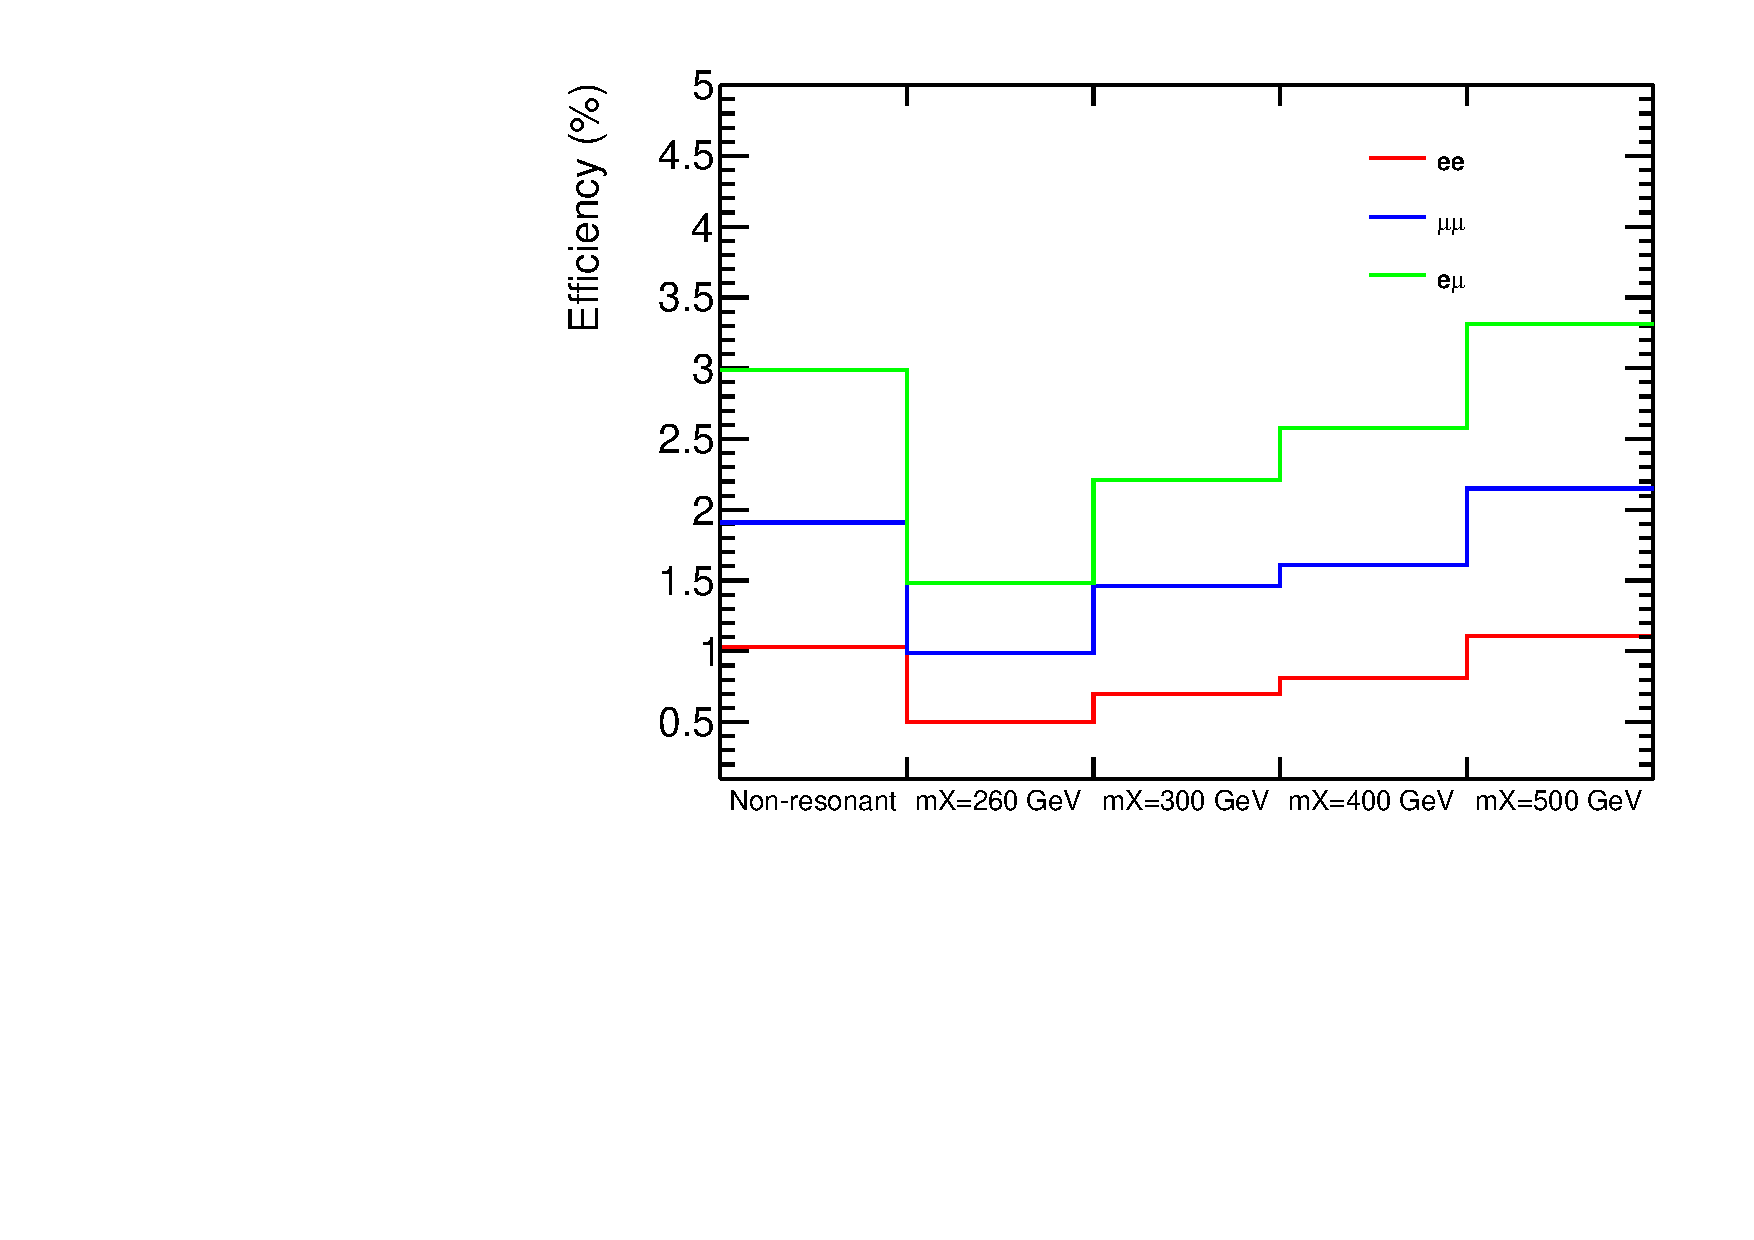
\includegraphics[width=0.55\textwidth, angle =-90]{fig/SigTopo/eff_presel_hh.pdf}
%\caption{The final efficiency of pre-selections for $hh$ signal samples.}
\caption{$hh$ MC的初步筛选效率。}
\label{fig:eff_pre_sel_hh}
\end{figure}

\begin{figure}
\centering
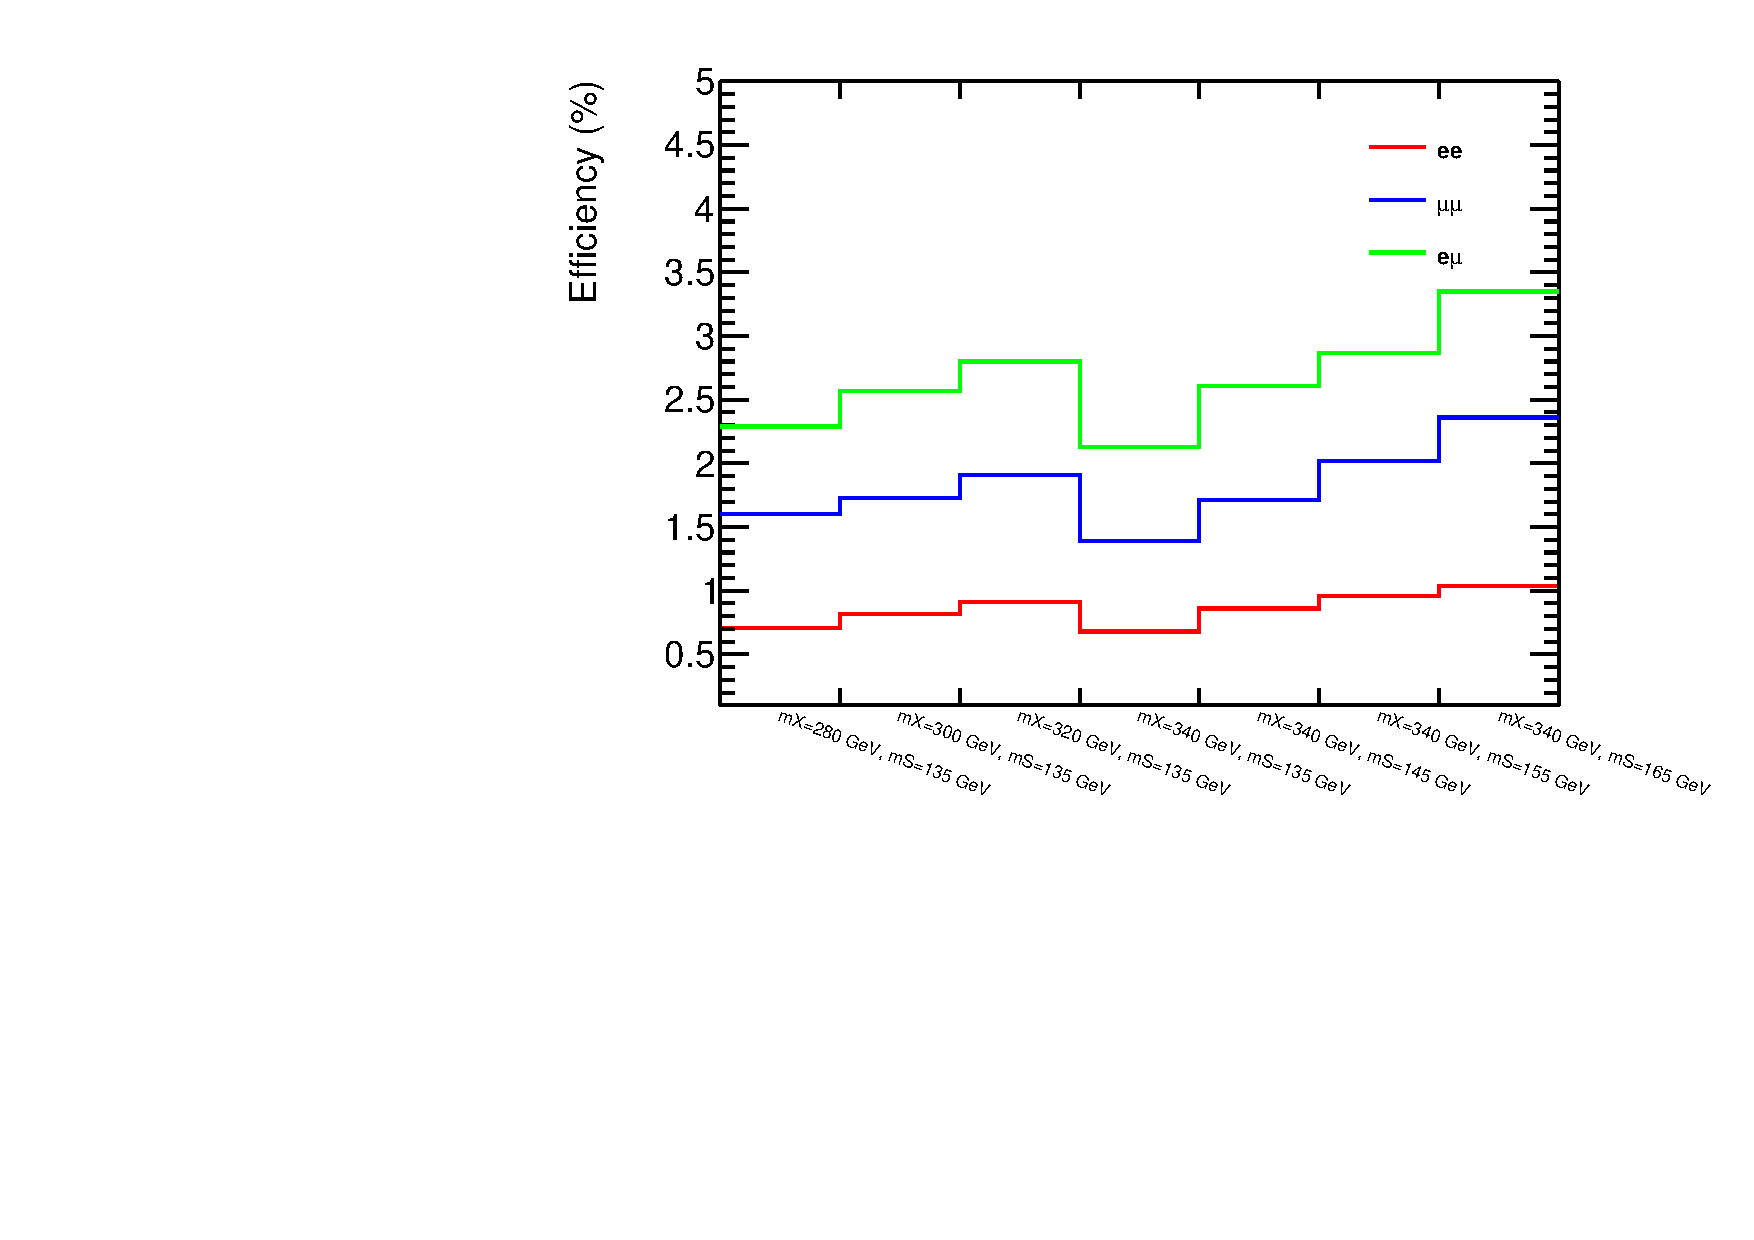
\includegraphics[width=0.55\textwidth, angle =-90]{fig/SigTopo/eff_presel_SS.pdf}
%\caption{The final efficiency of pre-selections for $SS$ signal samples.}
\caption{$SS$ MC的初步筛选效率。}
\label{fig:eff_pre_sel_SS}
\end{figure}

\subsection{喷注数分类}
\subsubsection{$hh$喷注数分类}\label{subsubsec:hh_optimization}
本分析中的显著信号是两个相同电荷的轻子。两个希格斯粒子倾向于出射到两个相反的半球,随后,两个希格斯粒子均衰变
到$W$玻色子,总共四个$W$玻色子中有两个是不在壳的,而不在壳的$W$玻色子会贡献相当部分的低动量的喷注(\pt < 25 GeV)。
在图~\ref{fig:SigTopo:pt_jet_mH260}到\ref{fig:SigTopo:pt_jet_nonres}中可以看到(此图未通过初步筛选条件),很大一部分的第四条喷注 \pt 是低于25 GeV的,甚至发生在高质量信号点。
加上基本的筛选条件之后,大部分信号事例只有三条喷注,如图\ref{fig:SigTopo:numOfjet_sig}所示。对于低质量点,即$m_X$=260 GeV 和$m_X$=300 GeV,其大部分事例最多只有2条喷注。
所以,对于不同的质量点,应当应用不同的喷注数条件,对于低质量点,要求$N_\text{jet}\ge$2,而对于高质量点,要求$N_\text{jet}\ge$3。
%为了证实该分类能够给出最高的信号显著性,考虑本底后,详细检查可见附录~\ref{app:}。
最后,一系列运动学变量被重建以用于信号优化(以及本底估计验证),具体优化方法会在章节~\ref{sec:signal_optimization}讨论。
以下列出一些能够较好区分信号与本底的变量:
\begin{itemize}
 \item $M(\ell\ell)$, 双轻子的不变质量;
 %\item $MET$, missing transverse energy;
 \item $M(jj)^W$, 两个距离最近喷注的不变质量;%the invariant mass of two closest jets among all selected good jets;
 \item $M(l_1jj)$, 领头轻子与两个距离最近喷注的不变质量;%the invariant mass of leading lepton and two closest jets;
 \item $M(all)$, 所有粒子的不变质量;%the invariant mass of all selected objects;
 \item $M_T$, 所有粒子的横向质量;%the transverse mass of all selected objects;
 \item $\Delta R_{min}(\ell_1, j)$, 领头轻子与最近喷注的角距离;%distance between leading lepton and the closest jet;
 \item $\Delta R_{min}(\ell_2, j)$, 次领头轻子与最近喷注的角距离。%distance between sub leading lepton and the closest jet;
\end{itemize}

\begin{figure}
\centering
\begin{subfigure}[b]{0.45\textwidth}
 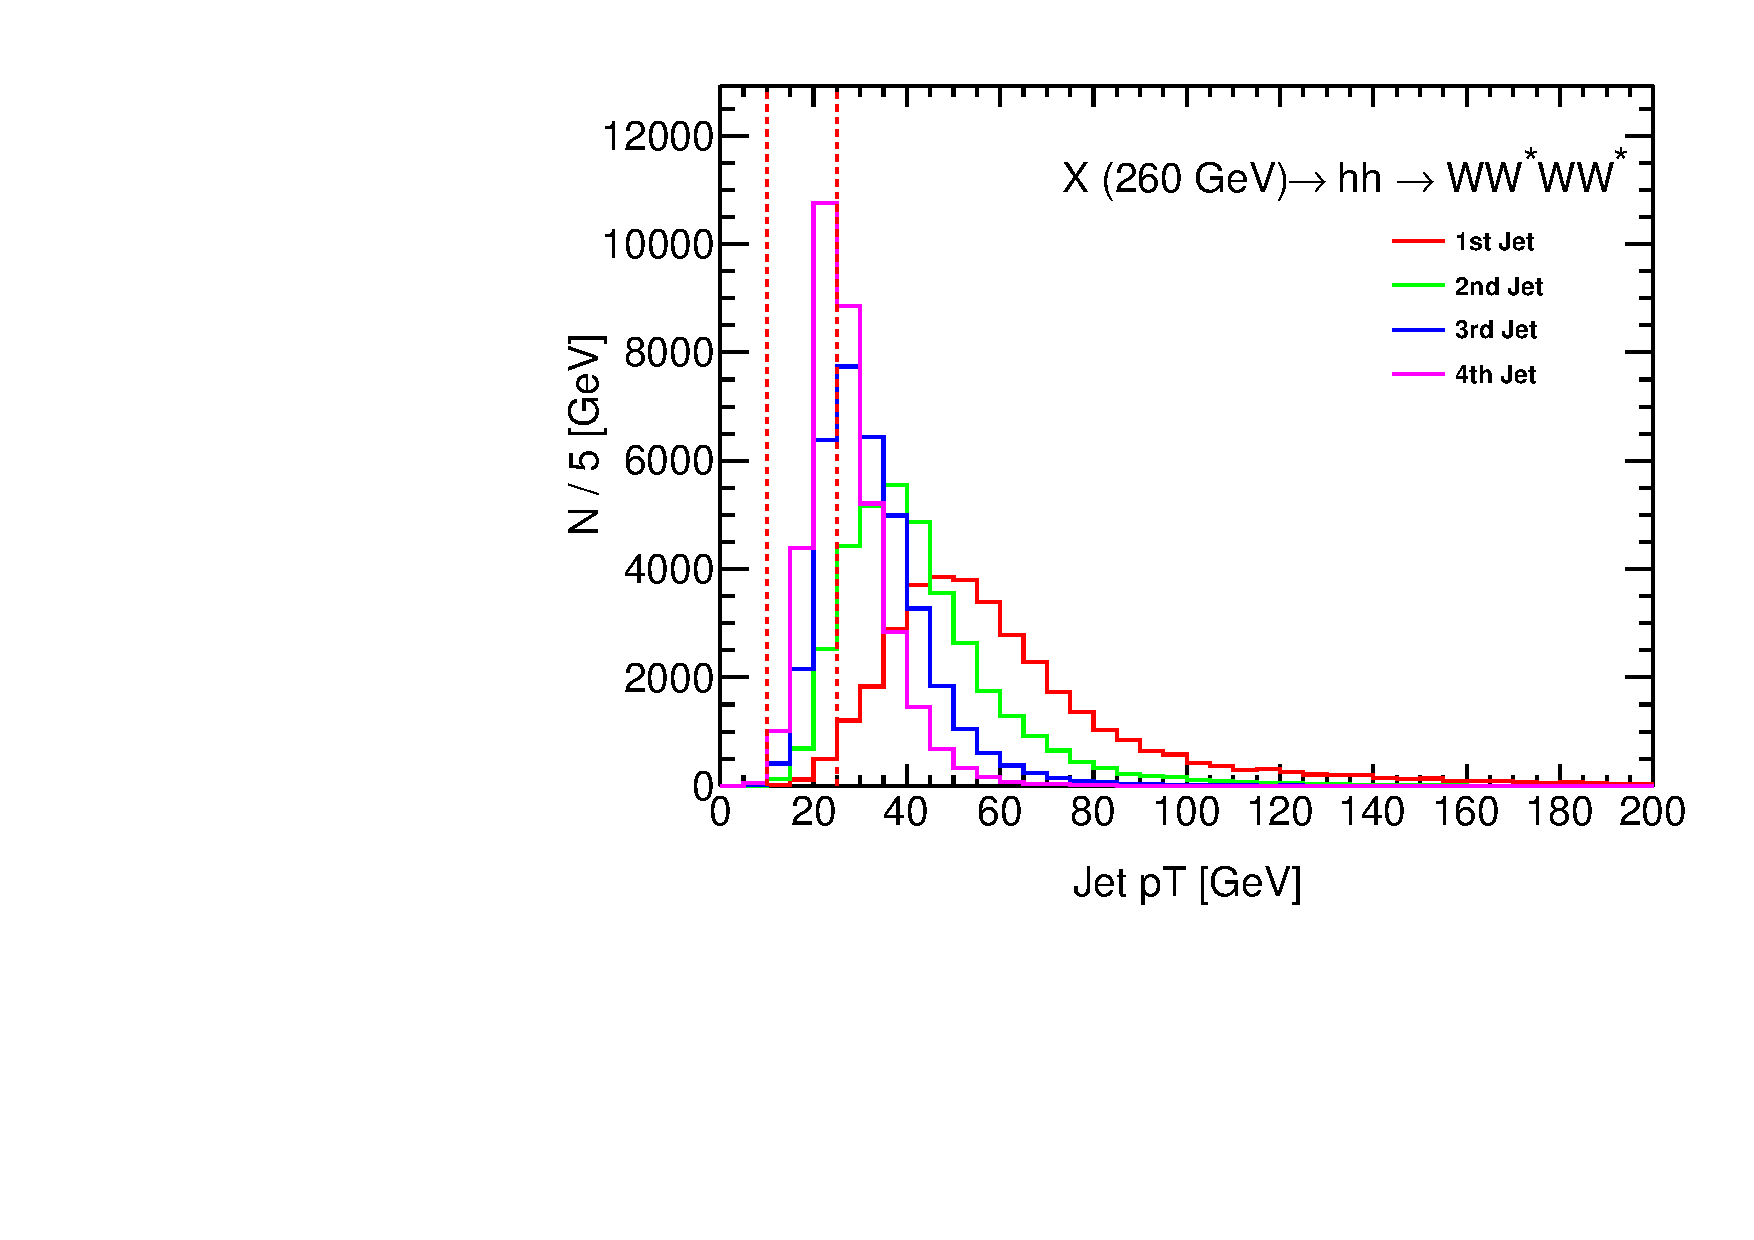
\includegraphics[width=0.75\textwidth, angle =-90]{fig/SigTopo/pt_jet_mH260.pdf}\caption{}
 \label{fig:SigTopo:pt_jet_mH260}
\end{subfigure}
\begin{subfigure}[b]{0.45\textwidth}
 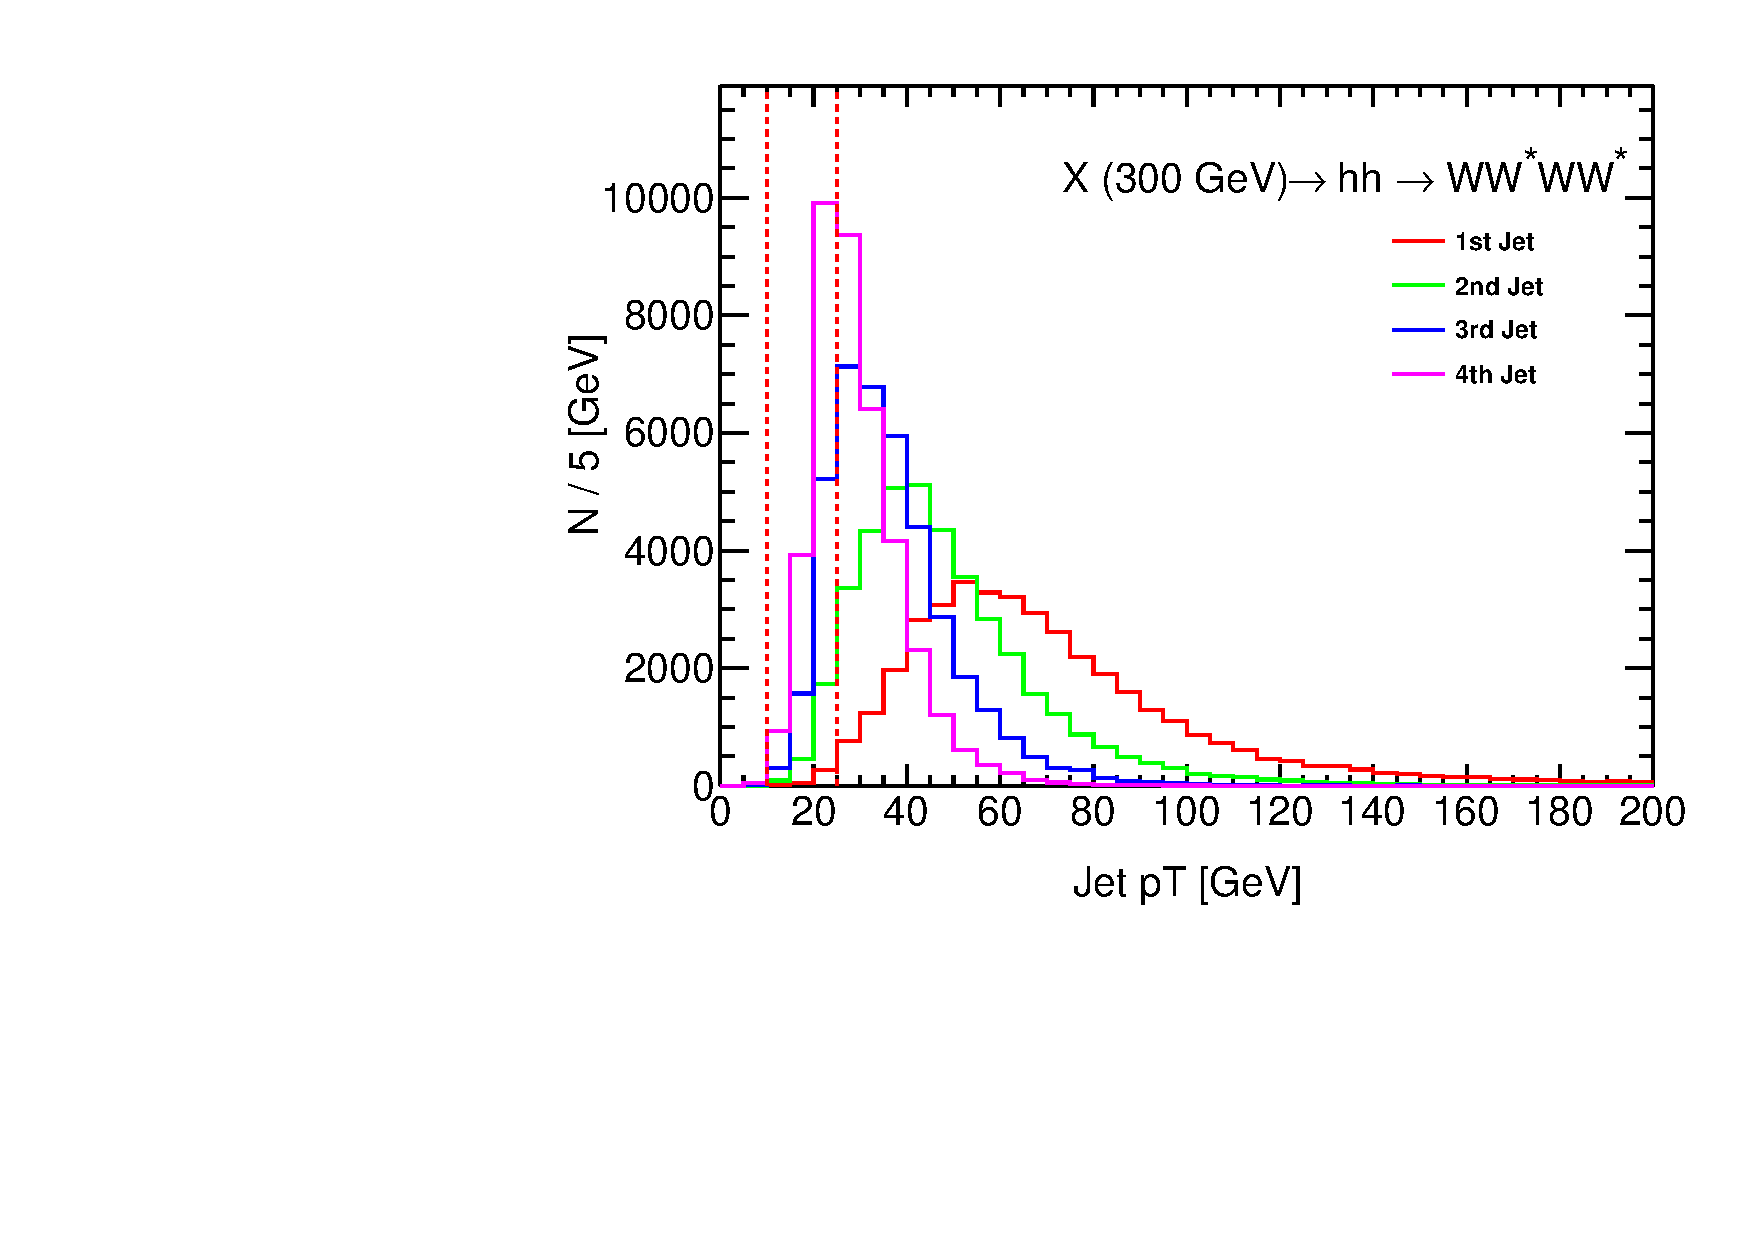
\includegraphics[width=0.75\textwidth, angle =-90]{fig/SigTopo/pt_jet_mH300.pdf}\caption{}
 \label{fig:SigTopo:pt_jet_mH300}
\end{subfigure}
\begin{subfigure}[b]{0.45\textwidth}
 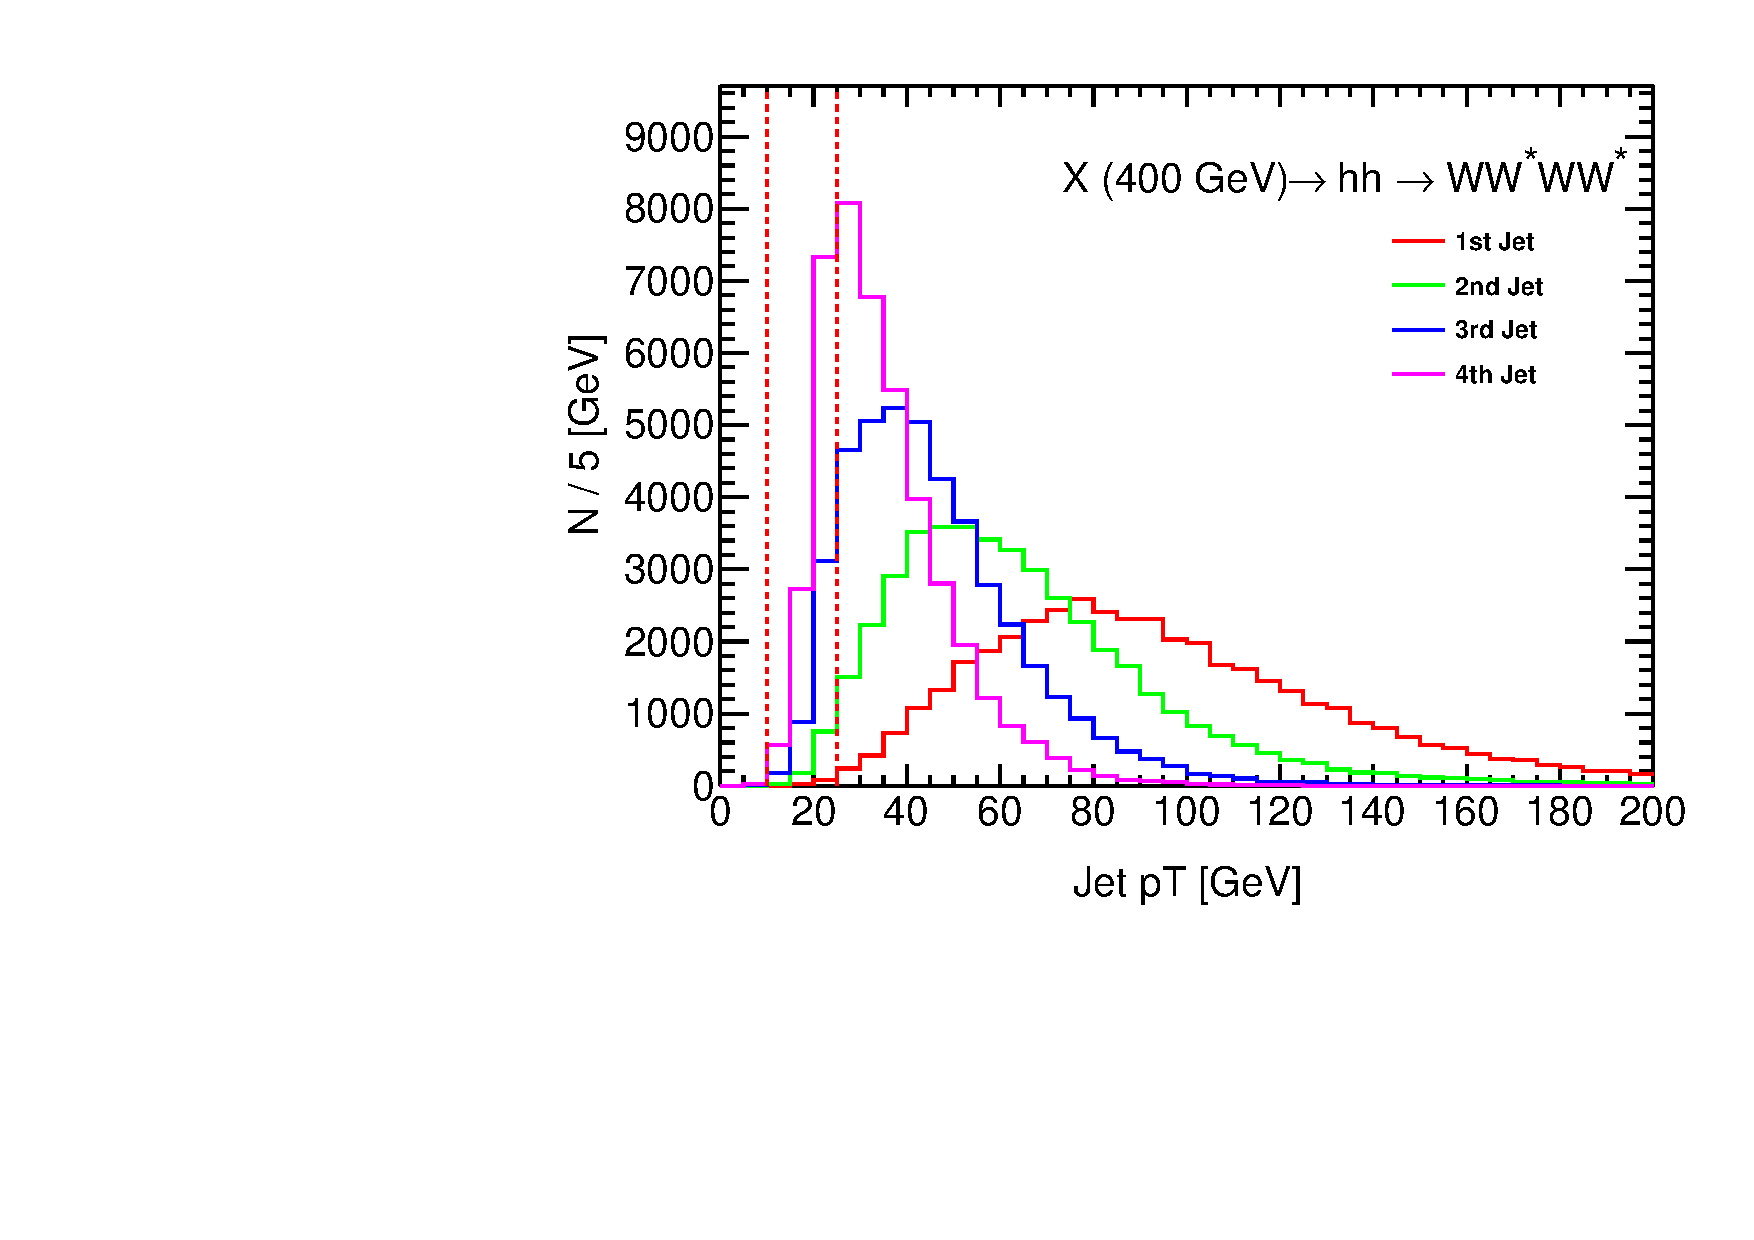
\includegraphics[width=0.75\textwidth, angle =-90]{fig/SigTopo/pt_jet_mH400.pdf}\caption{}
 \label{fig:SigTopo:pt_jet_mH400}
\end{subfigure}
\begin{subfigure}[b]{0.45\textwidth}
 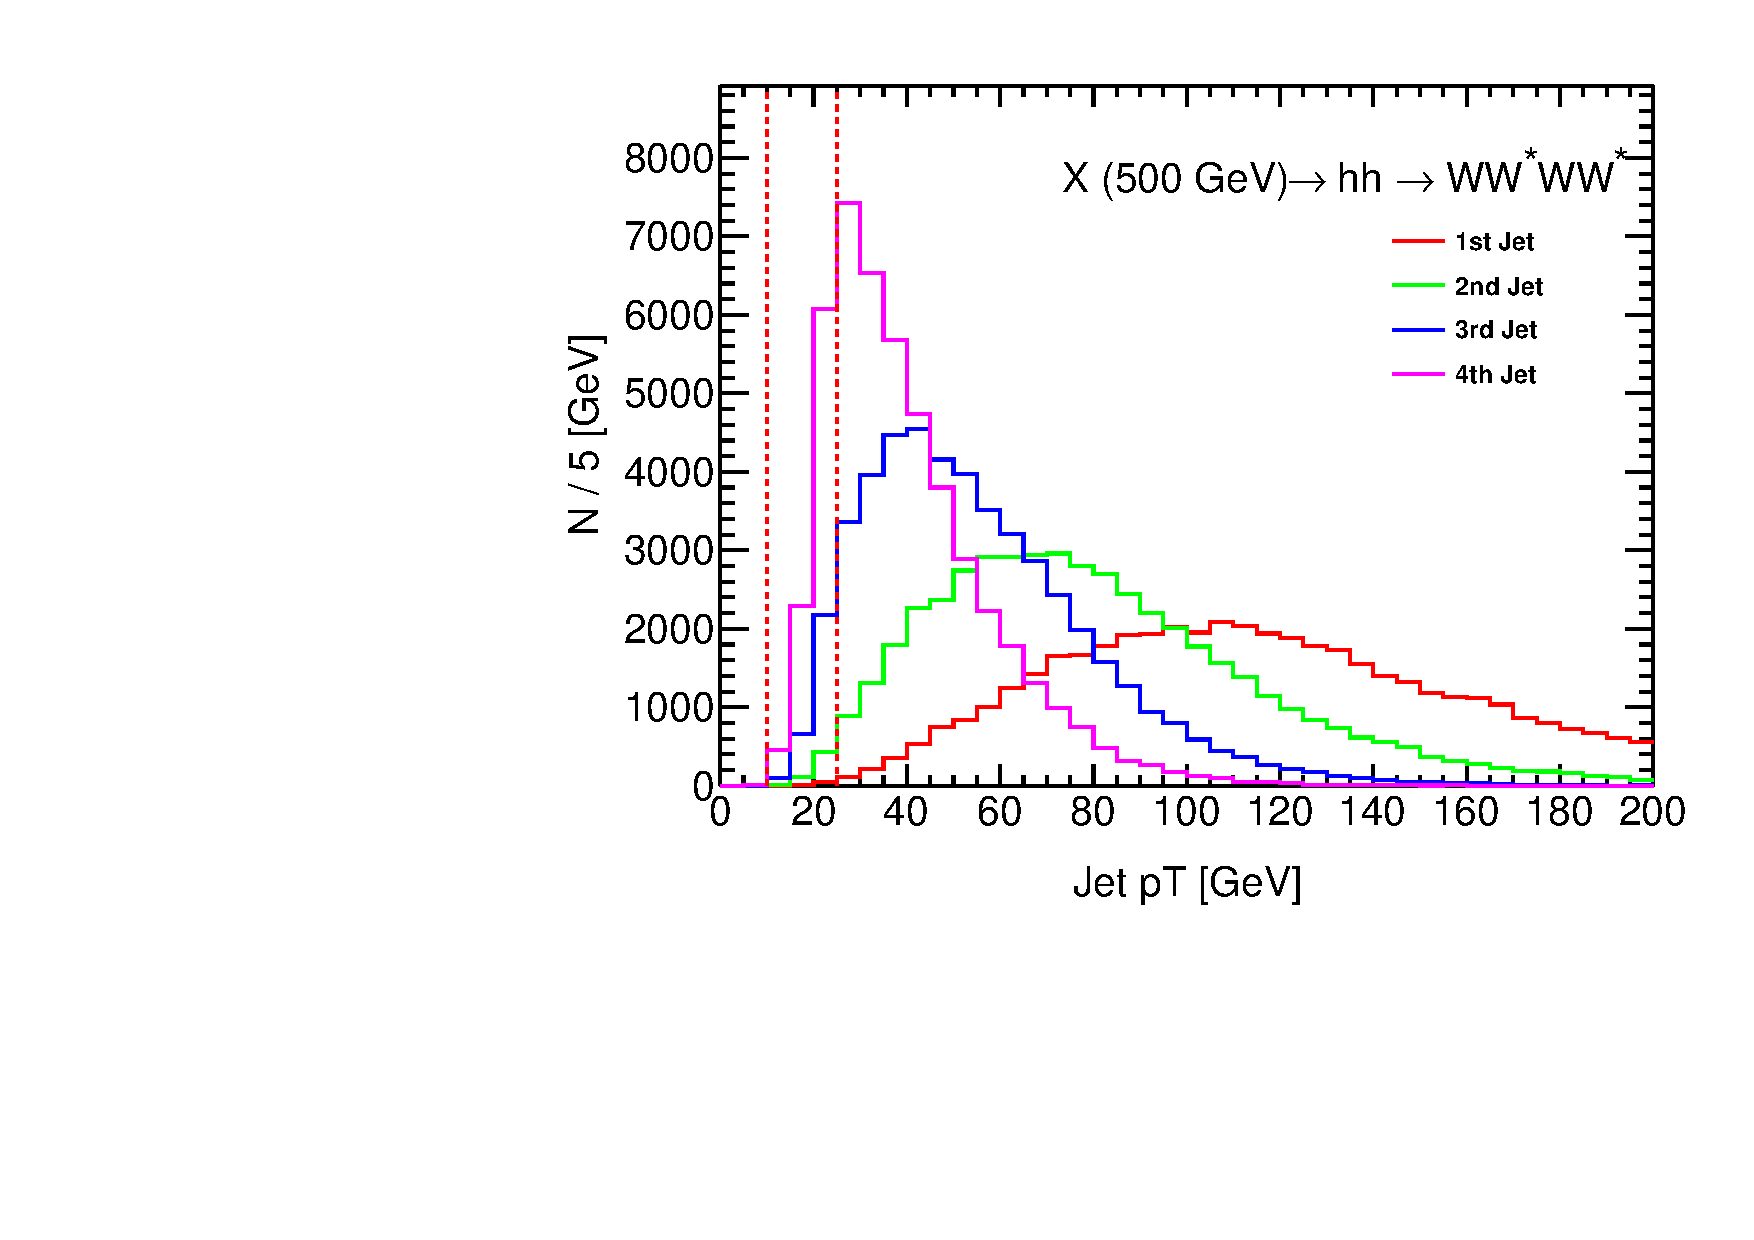
\includegraphics[width=0.75\textwidth, angle =-90]{fig/SigTopo/pt_jet_mH500.pdf}\caption{}
 \label{fig:SigTopo:pt_jet_mH500}
\end{subfigure}
\begin{subfigure}[b]{0.45\textwidth}
 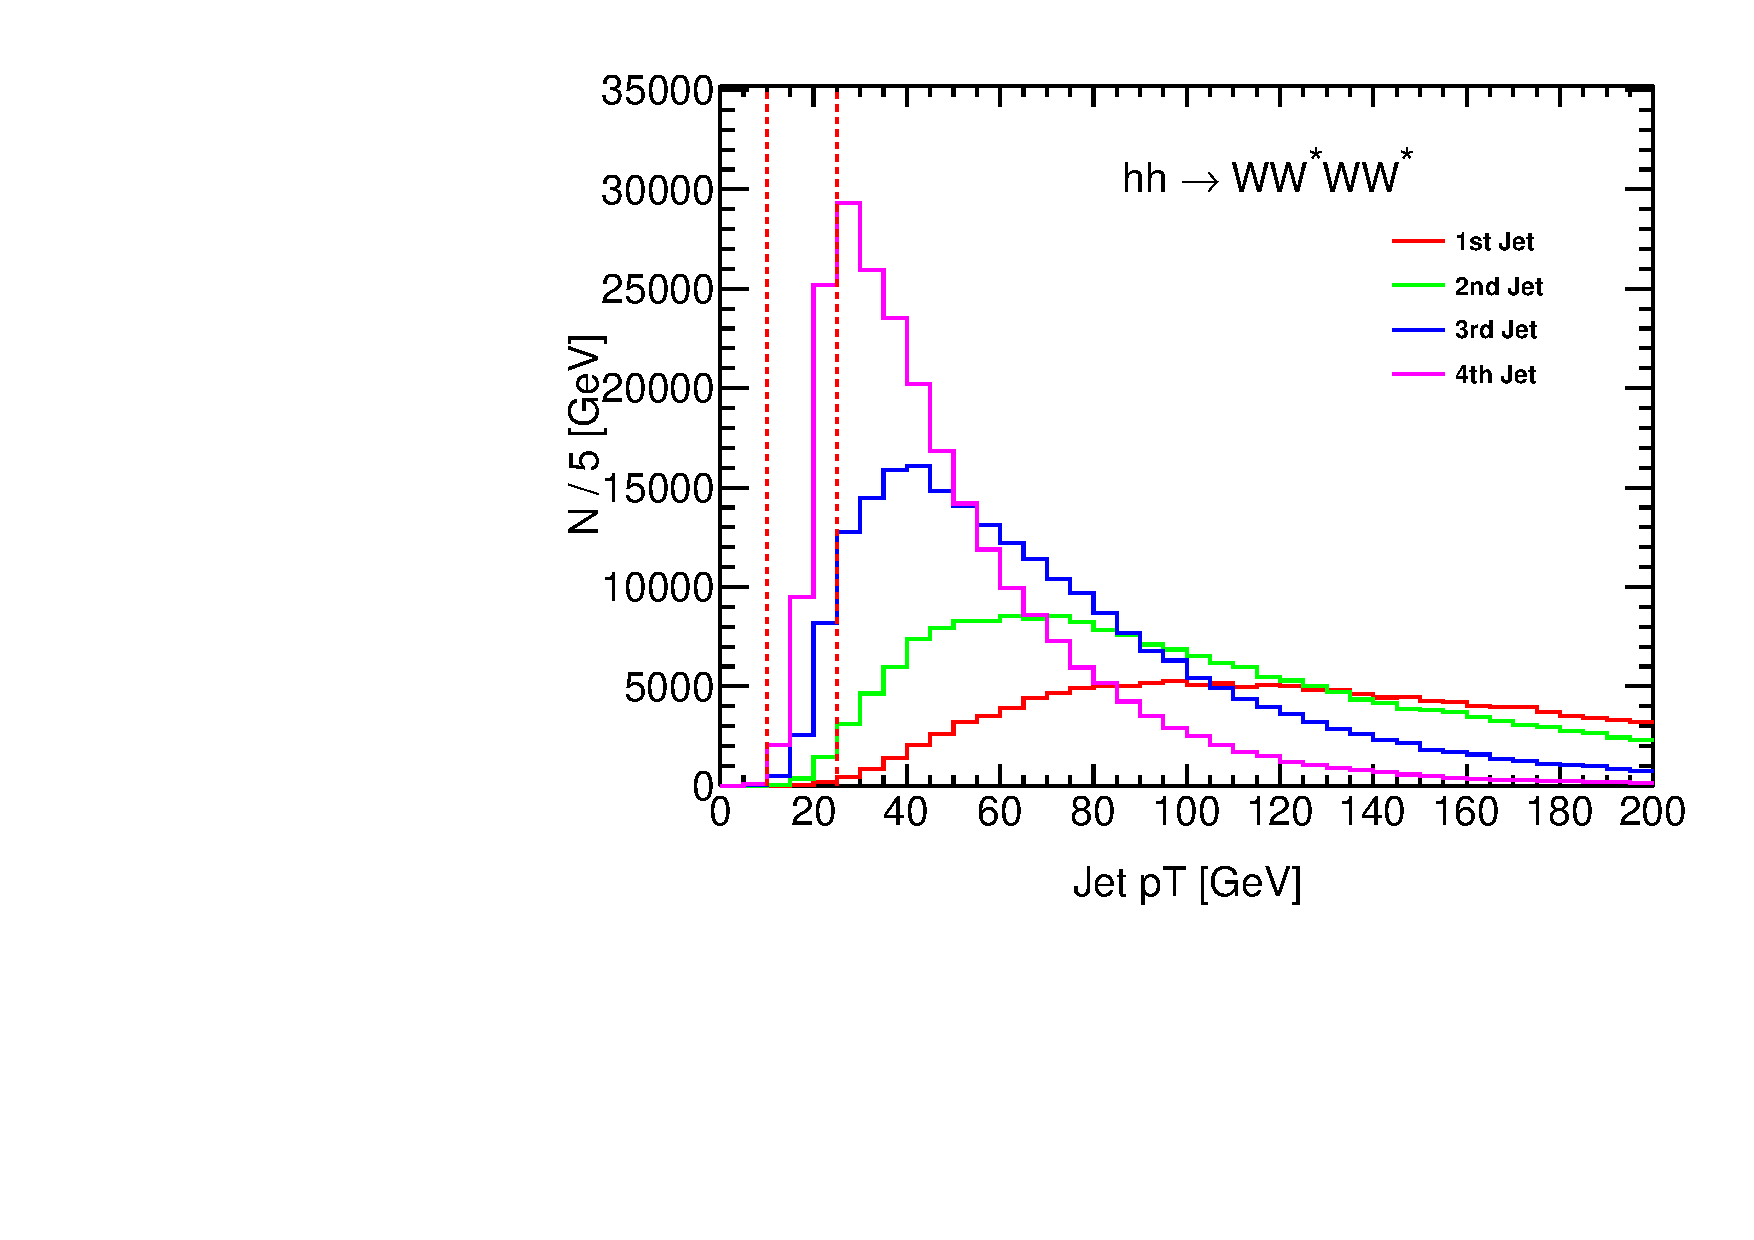
\includegraphics[width=0.75\textwidth, angle =-90]{fig/SigTopo/pt_jet_nonres.pdf}\caption{}
 \label{fig:SigTopo:pt_jet_nonres}
\end{subfigure}
\begin{subfigure}[b]{0.45\textwidth}
 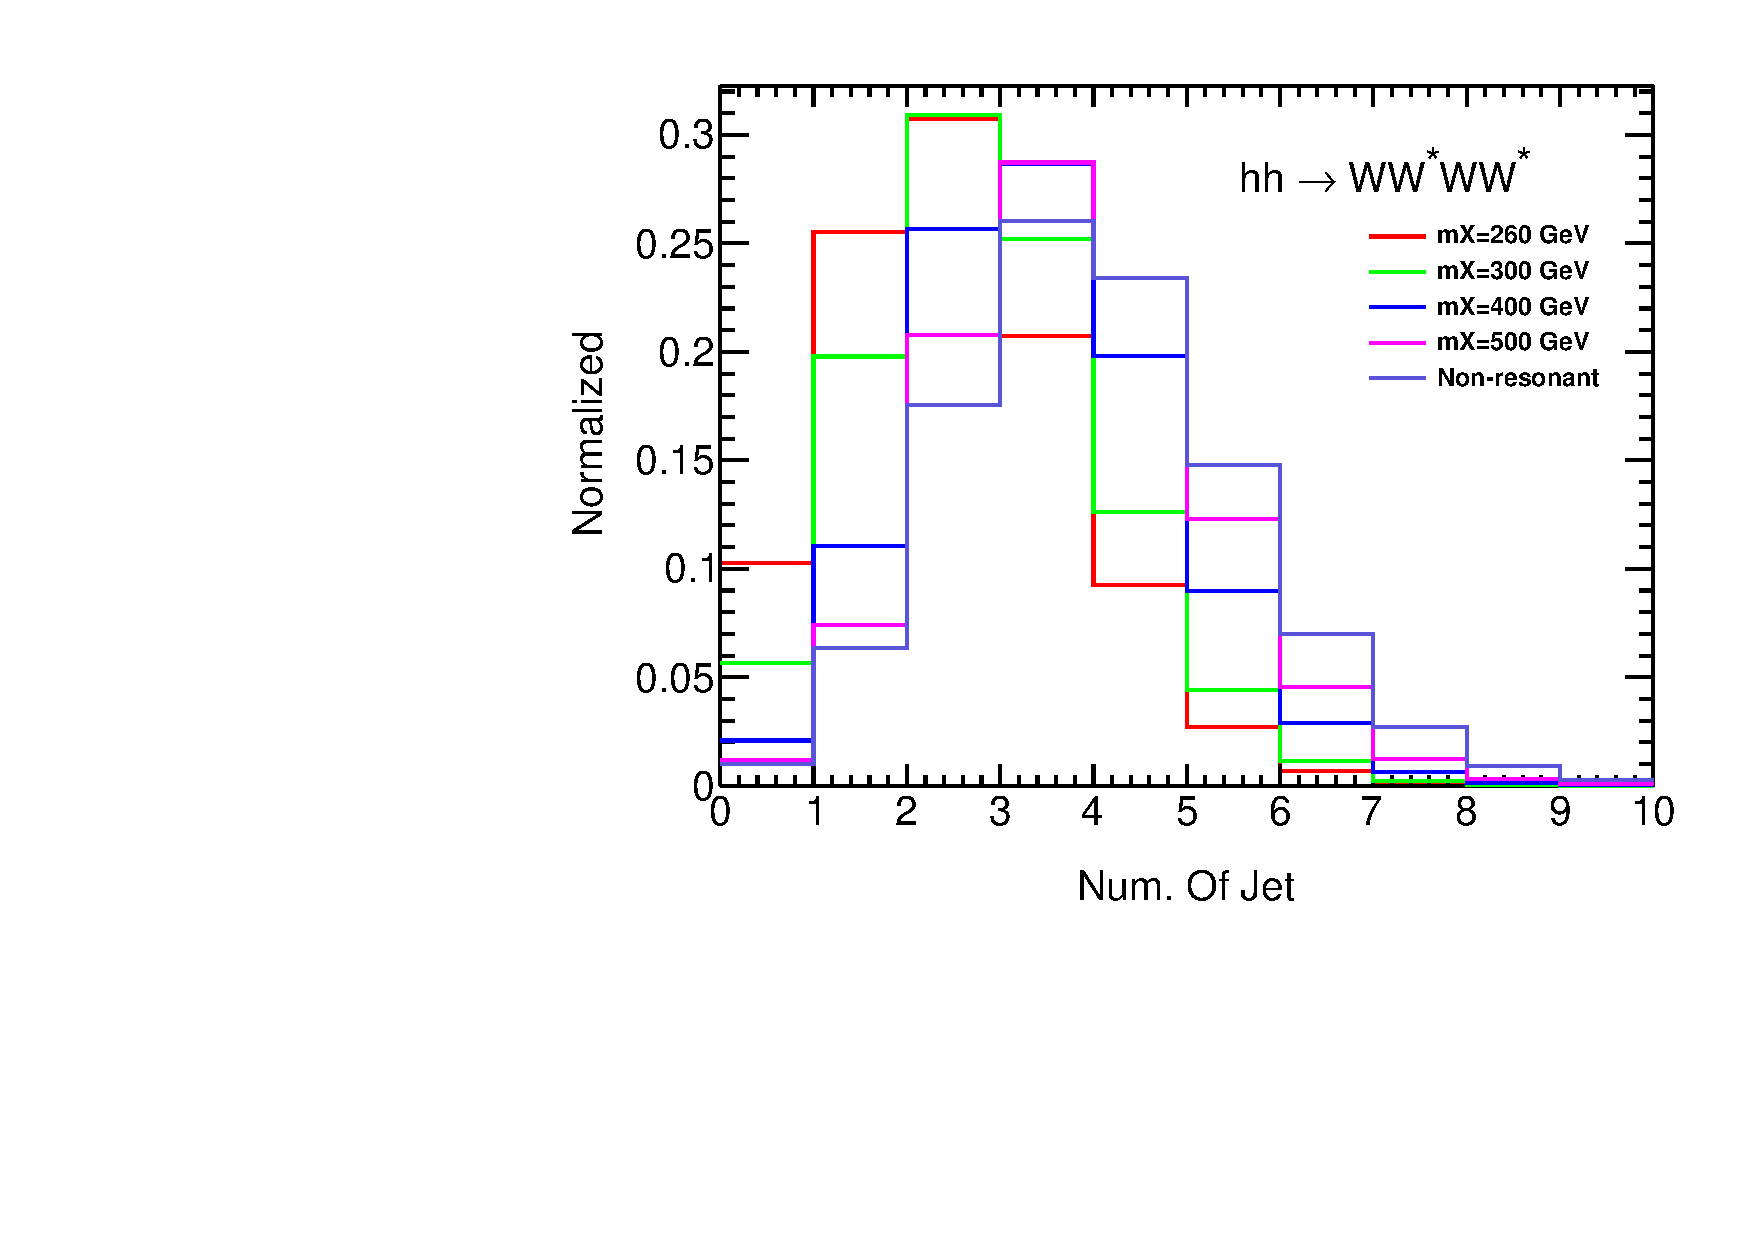
\includegraphics[width=0.75\textwidth, angle =-90]{fig/SigTopo/numOfjet_sig.pdf}\caption{}
 \label{fig:SigTopo:numOfjet_sig}
\end{subfigure}
\caption{$hh$信号的喷注\pt 分布和喷注数分布。图\ref{fig:SigTopo:pt_jet_mH260}到\ref{fig:SigTopo:pt_jet_nonres}是不同质量点的喷注未加$\pt>25$ GeV条件之前的\pt 分布,红色虚线分别对应\pt =10 GeV和\pt =25 GeV。图\ref{fig:SigTopo:numOfjet_sig}是喷注加上$\pt>25$ GeV条件之后的喷注数分布。}
%Distributions of $p_T$ and number of jet for signal. Figure~\ref{fig:SigTopo:pt_jet_mH260} to Figure~\ref{fig:SigTopo:pt_jet_nonres} are distributions of $p_T$ of jet before 25 GeV cuts, corresponding for mX=260, 300, 400, 500 GeV and non-resonant signal. Two dashed vertical lines are $p_T$=10 GeV and $p_T$=25 GeV, respectively. Figure~\ref{fig:SigTopo:numOfjet_sig} is number of jet distribution after 25 GeV cuts.}
\label{fig:SigTopo:pt_jet}
\end{figure}

\subsubsection{$SS$喷注数分类}
$S$标量粒子所取质量从135 GeV到165 GeV,$X$粒子从280 GeV到340 GeV。$SS$与$hh$具有类似的动力学性质,为了尽可能增加信号信号显著性,$N_\text{jet}$分类适用于此,具体如下:
\begin{itemize}
 \item 固定$m_S=135$~GeV: $m_X=280$~GeV, $m_X=300$~GeV and $m_X=320$~GeV; $N_{\text{jet}}\geq$2。
 \item 固定$m_X=340$~GeV: $m_S=135$~GeV, $m_S=145$~GeV, $m_S=155$~GeV and $m_S=165$~GeV; $N_{\text{jet}}\geq$3。
\end{itemize}
前述章节~\ref{subsubsec:hh_optimization}的动力学变量也可用于信号优化。
